\documentclass[tikz]{standalone}
\usepackage{pgfplots}
\pgfplotsset{compat=1.15}
\usepackage{mathrsfs}
\usetikzlibrary{arrows,calc}
\usepackage{tkz-euclide}

\pagestyle{empty}

\definecolor{AngleClr}{rgb}{0,0.39215686274509803,0}
\definecolor{ShapeClr}{rgb}{0.6,0.2,0}
\definecolor{BlueClr}{RGB}{13,93,184}

\begin{document}

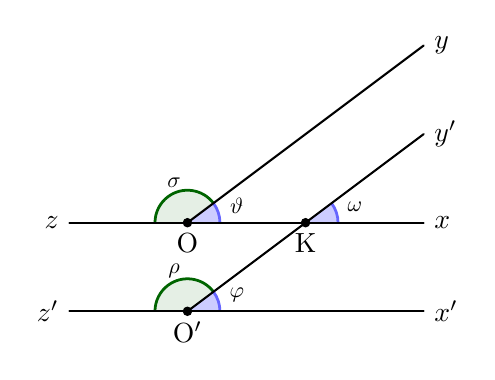
\begin{tikzpicture}[scale=.75]
\tkzSetUpLine[line width=1pt,color=black]
\tkzSetUpPoint[fill=black]

\tkzDefPoints{0/0/z,0/-1.5/z',2/0/O,2/-1.5/O',6/0/x,6/-1.5/x',6/3/y,6/1.5/y'}

\tkzInterLL(z,x)(O',y') \tkzGetPoint{K}

\tkzFillAngles[fill=AngleClr,size=.55,fill opacity=0.1](y,O,z)
\tkzMarkAngles[line width=1pt,size=.55,color=AngleClr](y,O,z)
\tkzLabelAngles[scale=0.8,pos=0.9](y,O,z){$\sigma$}

\tkzFillAngles[fill=blue!20!white,size=.55](x,O,y)
\tkzMarkAngles[line width=1pt,size=.55,color=blue!60!white](x,O,y)
\tkzLabelAngles[scale=0.8,pos=1.1](x,O,y){$\vartheta$}

\tkzFillAngles[fill=blue!20!white,size=.55](x',O',y')
\tkzMarkAngles[line width=1pt,size=.55,color=blue!60!white](x',O',y')
\tkzLabelAngles[scale=0.8,pos=1.1](x',O',y'){$\varphi$}

\tkzFillAngles[fill=AngleClr,size=.55,fill opacity=0.1](y',O',z')
\tkzMarkAngles[line width=1pt,size=.55,color=AngleClr](y',O',z')
\tkzLabelAngles[scale=0.8,pos=0.9](y',O',z'){$\rho$}

\tkzFillAngles[fill=blue!20!white,size=.55](x,K,y')
\tkzMarkAngles[line width=1pt,size=.55,color=blue!60!white](x,K,y')
\tkzLabelAngles[scale=0.8,pos=1.1](x,K,y'){$\omega$}

\tkzDrawSegment[line width=0.75pt](z,x)
\tkzDrawSegment[line width=0.75pt](z',x')
\tkzDrawSegment[line width=0.75pt](O,y)
\tkzDrawSegment[line width=0.75pt](O',y')

\tkzDrawPoints[size=3](O,O',K)

\tkzLabelPoint[below](O){$\rm O$}
\tkzLabelPoint[below](O'){$\rm O'$}
\tkzLabelPoint[below](K){$\rm K$}

\tkzLabelPoint[left](z){$z$}
\tkzLabelPoint[left](z'){$z'$}
\tkzLabelPoint[right](x){$x$}
\tkzLabelPoint[right](x'){$x'$}

\tkzLabelPoint[right](y){$y$}
\tkzLabelPoint[right](y'){$y'$}


\end{tikzpicture}

\end{document}